\begin{SCtable}[][b]
    \centering
    \begin{tabular}{c c c}
        \multicolumn{3}{c}{\textbf{Lunghezze, periodi e accelerazione ricavata}} \\
        \toprule
        Lunghezza [\si{\metre}] & Periodi [\si{\second}] & Accelerazione [\si{\metre\per\square\second}] \\ %di gravità
        $\ell_i$ & $\mathcal{T}_i \pm \delta\mathcal{T}_i$ & $g_i \pm \delta g_i$ \\
        \midrule
			1.052 & 2.061 $\,\pm\,$ 0.006 & 9.8 $\,\pm\,$ 0.1 \\
			0.949 & 1.947 $\,\pm\,$ 0.004 & 9.87 $\,\pm\,$ 0.08 \\
			0.849 & 1.856 $\,\pm\,$ 0.003 & 9.72 $\,\pm\,$ 0.06 \\
			0.749 & 1.739 $\,\pm\,$ 0.003 & 9.77 $\,\pm\,$ 0.07 \\
			0.649 & 1.610 $\,\pm\,$ 0.003 & 9.88 $\,\pm\,$ 0.08 \\
			0.549 & 1.477 $\,\pm\,$ 0.005 & 9.9 $\,\pm\,$ 0.1 \\
			0.449 & 1.335 $\,\pm\,$ 0.004 & 9.9 $\,\pm\,$ 0.1 \\
			0.349 & 1.187 $\,\pm\,$ 0.004 & 9.8 $\,\pm\,$ 0.1 \\
			0.249 & 1.008 $\,\pm\,$ 0.004 & 9.7 $\,\pm\,$ 0.1 \\
			0.149 & 0.778 $\,\pm\,$ 0.004 & 9.7 $\,\pm\,$ 0.2 \\
		\bottomrule
    \end{tabular}
    \caption{In questa tebella sono riportate nella prima colonna le misure della lunghezza del filo che sono tutte affette da un'incertezza di 0.0006 m ricavata nel paragrafo precedente al punto \ref{l_medie}. Nella seconda colonna sono riportati i valori medi del periodo di oscillazione del pendolo relativo a ciascuna lunghezza. Infine nella terza colonna sono riportati i valori di $g_i$ derivanti dai dati grazie alle equazioni (\ref{eq:g}) e (\ref{eq:delta_g}). Per maggiori informazioni sulle prime due colonne si faccia riferimento alla Tabella \ref{tab:l_dati}, che commenta anche l'origine delle misure e la loro incertezza.}
    \label{tab:calcolo_g}
\end{SCtable}

Facendo riferimento ai valori sperimentali dell'allungamento, $\ell_i$, e del periodo, $\mathcal{T}_i$, riportati nella tabella \ref{tab:calcolo_g} vogliamo calcolare una stima dell'accelerazione di gravità, $g_i$, per ognuno di essi sfruttando la relazione (\ref{eq:g}). Inoltre sappiamo che il valore così rovato di $g$ non è assoluo ma è affetto da un incertezza $\delta g_i$ che possiamo stimare sfruttando la formula generale per la propagazione degli errori, ovvero:

\begin{equation*}
(\delta g)^2 \, \simeq \, \left( \frac{\partial g}{\partial \ell} \right)^2 (\delta \ell)^2 \, + \, \left( \frac{\partial g}{\partial \mathcal{T}} \right)^2 (\delta \mathcal{T})^2
\end{equation*}
%
Pertanto sapendo che:

\begin{equation*}
(\delta g)^2 \, \simeq \, \left( \frac{2 \pi}{\mathcal{T}} \right)^4 (\delta \ell)^2 \, + \, \left( \frac{8 \pi^2 \ell}{\mathcal{T}^3} \right)^2 (\delta \mathcal{T})^2
\end{equation*}
%
e quindi, possiamo riassumere che l'incertezza sul valore sperimentale dell'accelerazione di gravità relativo ad ogni singola misura è il seguente:

\begin{equation} \label{eq:delta_g}
\delta g \,\, \simeq \,\, \sqrt{\left( \frac{2 \pi}{\mathcal{T}} \right)^4 (\delta \ell)^2 \,\, + \,\, \left( \frac{8 \pi^2 \ell}{\mathcal{T}^3} \right)^2 (\delta \mathcal{T})^2}
\end{equation}
%
Sempre analizzando i dati da noi raccolti ci possiamo accorgere che le incertezze relative alla misura della lunghezza del pendolo sono minori di un ordine di grandezza rispetto alle incertezze relative al periodo.
%Ciononostante, esaminando la formula (\ref{eq:delta_g}), si osserva una dipendenza dell'incertezza $d_g$ dal valore di $\ell$. Infatti per $\ell$ piccoli si osserva che $\delta \ell$ ha una influenza maggiore di  $\delta \mathcal{T}$ nel calcolo di $d_g$, mentre per  $\ell$ grandi si osserva l'opposto.

%WARNING! Controllare la correttezza della precedente affermazione $\bigotimes$
%Ciononostante, esaminando la formula (\ref{eq:delta_g}), si può notare come al decrescere del valore di $\ell_i$ diminusica l'influenza di $\delta\mathcal{T}$ e aumenti quella di $\delta\ell$.

\begin{SCfigure}
	\centering
	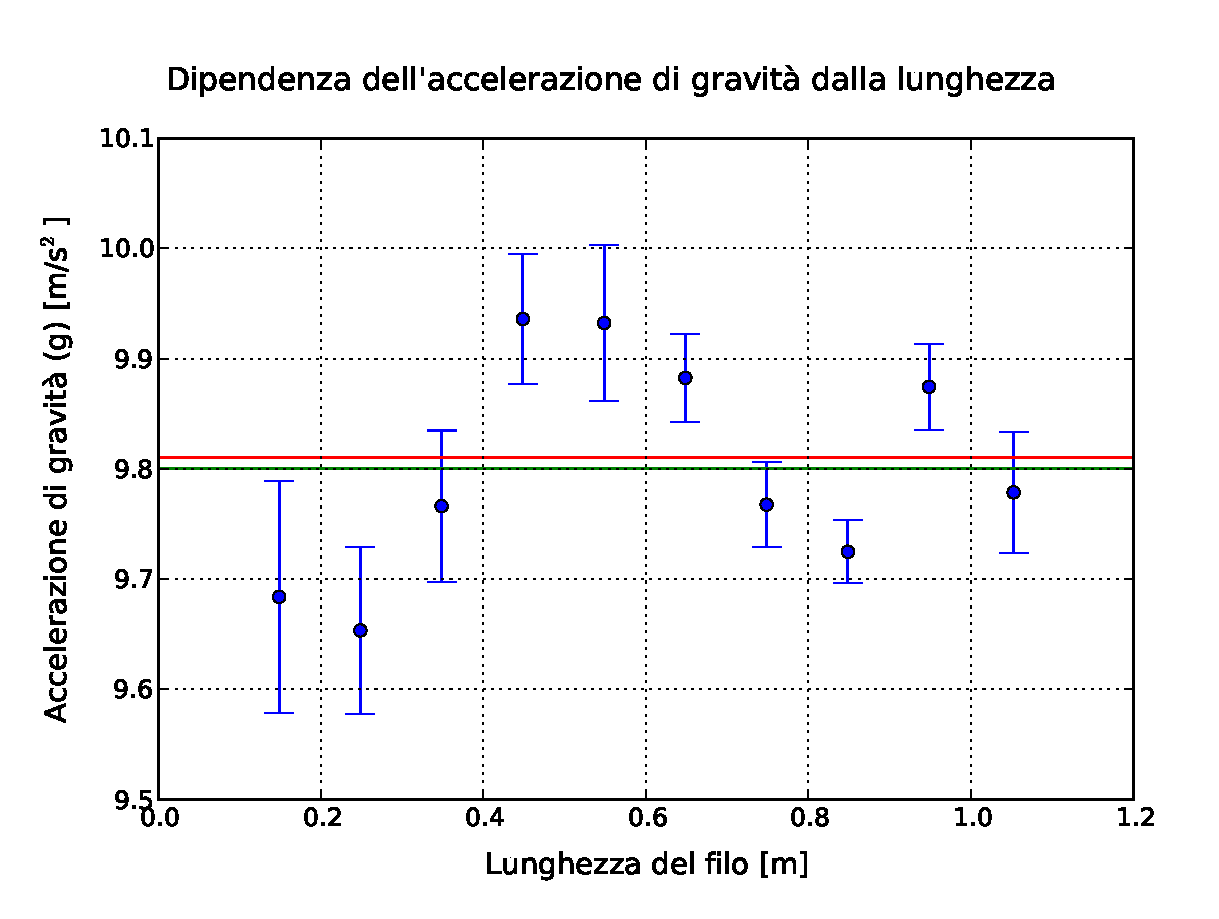
\includegraphics[width=120mm]{immagini/gravita.pdf}
	\caption{Il grafico rappresenta la dipendenza dell'accelerazione di gravità dalla lunghezza del pendolo, evidenziando le incertezze relative ad ogni valore. Si può notare come le incertezze relative a $\ell$ minori siano in genere più elevate rispetto a quelle relative a $\ell$ maggiori. Non è possibile osservare alcun andamento residuo, ad esclusione del celeberrimo andamento residuo a dinosauro.}
	\label{fig:graf_gravita}
\end{SCfigure}

Dai valori di $g_i$ ottenuti possiamo notare che questi risultano essere differenti tra di loro. Sicuramente una causa di questa diversità si può attribuire agli errori sistematici, in quanto le misure del periodo di oscillazione del pendolo sono state effettuate tutte da uno stesso operatore, e quindi i dati sperimentali possono essere affetti da un errore sistematico dovuto in parte alla prontezza di riflessi dell'operatore. %(In questo caso bisogna incolpare il nostro compagno davide Bazzanella per non essere riuscito a fare delle misure abbastana esatte del periodo da restituirci un valore di g spaccato con la predizione teorica!!! CATTIVO DAVIDE!!!).
% che simpaticoni xD LeL
Osservando il grafico in Figura \ref{fig:graf_gravita} non siamo in grado di affermare che i vari valori assunti da $g_i$ si possano attribuire ad un errore di natura sistematica, ad esempio da una dipendenza dalla lunghezza del filo o del periodo, in quanto non si può dire che in questi vi sia un andamento residuo.\\
Nonostante quanto detto sopra, ovvero che non si può osservare un andamento residuo dei dati dal grafico, possiamo dire che per il modello che abbiamo adottato nell'eseguire l'esperienza, ovvero quello di pendolo semplice dove il filo ha una massa trascurabile, e la massa applicata è concentrata in un solo punto, sarebbe necessario che la lunghezza del filo risultasse essere abbastanza maggiore rispetto all'altezza della massa appesa. Pertanto non ci sentiamo di escludere del tutto che le misure più accurate dell'accelerazione di gravità possano essere quelle prese per lunghezze $\ell$ del filo maggiori, ovvero quando le dimensioni della massa applicata sono più trascurabili.
